% =====================================================================
%  MCMP117 -- Fundamentals of Operating Systems
%  Week 6 Course Notes: Memory Management: Contiguous Allocation, Paging & Segmentation
%  Compile with XeLaTeX (twice):  xelatex MCMP117_Week6_Notes.tex
%  Needs ./figures/ and the ../code/ folder.
% =====================================================================
\documentclass[11pt,a4paper]{article}
\newcommand{\weeknum}{6}
% ---------- Page & fonts ---------------------------------------------
\usepackage[a4paper,margin=2.3cm,headheight=15pt]{geometry}
\usepackage{fontspec}
\IfFontExistsTF{Calibri}{\setmainfont{Calibri}}{\setmainfont{Carlito}}
\IfFontExistsTF{Cambria}{\newfontfamily\headfont{Cambria}}{\newfontfamily\headfont{Caladea}}
\IfFontExistsTF{Consolas}{\setmonofont[Scale=0.95]{Consolas}}{\setmonofont[Scale=0.88]{DejaVu Sans Mono}}
\usepackage{amsmath,amssymb}
\usepackage{microtype}
\linespread{1.12}
\setlength{\parskip}{0.55em}
\setlength{\parindent}{0pt}

% ---------- Colours (course design system) ----------------------------
\usepackage{xcolor}
\definecolor{dark}{HTML}{212121}
\definecolor{charcoal}{HTML}{36454F}
\definecolor{slate}{HTML}{50808E}
\definecolor{mint}{HTML}{02C39A}
\definecolor{mintdeep}{HTML}{028090}
\definecolor{light}{HTML}{F2F2F2}
\definecolor{muted}{HTML}{6B7679}

% ---------- Packages ---------------------------------------------------
\usepackage{graphicx}
\usepackage{float}
\usepackage{needspace}
\graphicspath{{figures/}}
\usepackage[font=small,labelfont={bf,color=mintdeep},justification=centering]{caption}
\usepackage{booktabs,longtable,array,tabularx}
\usepackage{enumitem}
\setlist{itemsep=0.25em,topsep=0.3em}
\usepackage{tikz}
\usetikzlibrary{arrows.meta,positioning,calc,shapes.geometric}
\usepackage{pgfplots}
\pgfplotsset{compat=1.17}
\usepackage[most]{tcolorbox}
\usepackage{titlesec}
\usepackage{fancyhdr}
\usepackage{xurl}
\usepackage[colorlinks=true,linkcolor=mintdeep,urlcolor=mintdeep,citecolor=mintdeep]{hyperref}

% ---------- Headings ----------------------------------------------------
\titleformat{\section}{\headfont\Large\bfseries\color{charcoal}}{\color{mint}\thesection}{0.7em}{}
\titleformat{\subsection}{\headfont\large\bfseries\color{charcoal}}{\color{mintdeep}\thesubsection}{0.6em}{}
\titleformat{\subsubsection}{\headfont\normalsize\bfseries\color{mintdeep}}{}{0em}{}
\titlespacing*{\section}{0pt}{1.6em}{0.6em}
\titlespacing*{\subsection}{0pt}{1.2em}{0.4em}

% ---------- Header / footer -----------------------------------------------
\pagestyle{fancy}
\fancyhf{}
\fancyhead[L]{\small\color{muted}MCMP117 --- Fundamentals of Operating Systems}
\fancyhead[R]{\small\color{muted}Week \weeknum{} Notes}
\fancyfoot[C]{\small\color{muted}\thepage}
\renewcommand{\headrulewidth}{0pt}

% ---------- Boxes ---------------------------------------------------------
\newtcolorbox{keyidea}[1][Key idea]{enhanced,breakable,colback=charcoal,colframe=charcoal,
  coltext=white,fonttitle=\headfont\bfseries\color{mint},title={#1},
  attach title to upper={\par\smallskip},boxrule=0pt,arc=3pt,left=10pt,right=10pt,top=8pt,bottom=8pt}
\newtcolorbox{example}[1][Worked example]{enhanced,colback=light,colframe=light,
  fonttitle=\headfont\bfseries\color{mintdeep},title={#1},attach title to upper={\par\smallskip},
  boxrule=0pt,arc=3pt,left=10pt,right=10pt,top=8pt,bottom=8pt}
\newtcolorbox{tryit}[1][Try it yourself]{enhanced,breakable,colback=white,colframe=mint,
  fonttitle=\headfont\bfseries\color{mintdeep},title={#1},attach title to upper={\par\smallskip},
  boxrule=0.8pt,arc=3pt,left=10pt,right=10pt,top=8pt,bottom=8pt}
\newtcolorbox{histnote}[1][Historical note]{enhanced,breakable,colback=white,colframe=slate!40,
  fonttitle=\headfont\bfseries\color{slate},title={#1},attach title to upper={\par\smallskip},
  boxrule=0.5pt,arc=3pt,left=10pt,right=10pt,top=8pt,bottom=8pt,fontupper=\small}

% Photo helper: fits image inside a box, never distorted (keepaspectratio)
\newcommand{\photo}[3]{\includegraphics[width=#1,height=#2,keepaspectratio]{#3}}

\newcommand{\term}[1]{\textbf{\color{mintdeep}#1}}
\newcommand{\cmd}[1]{\texttt{#1}}


% ---------- Code listings ----------------------------------------------------
\usepackage{listings}
\lstdefinestyle{course}{
  basicstyle=\ttfamily\small, columns=fullflexible, keepspaces=true,
  backgroundcolor=\color{dark}, rulecolor=\color{dark}, frame=single, framesep=6pt,
  xleftmargin=8pt, xrightmargin=8pt, aboveskip=0.8em, belowskip=0.6em,
  basicstyle=\ttfamily\small\color{light},
  keywordstyle=\color{mint}\bfseries, commentstyle=\color{white!60}\itshape,
  stringstyle=\color{orange!70!yellow}, numberstyle=\tiny\color{muted},
  numbers=left, numbersep=10pt, showstringspaces=false, breaklines=true,
  tabsize=4, upquote=true}
\lstdefinestyle{term}{style=course, numbers=none, keywordstyle=\color{light},
  commentstyle=\color{white!60}, stringstyle=\color{light}}
\lstset{style=course,language=C}
\usepackage{textcomp}

\begin{document}
% ============================ Week 6 body ============================
\thispagestyle{empty}
\begin{tcolorbox}[enhanced,colback=dark,colframe=dark,arc=0pt,boxrule=0pt,
  left=18pt,right=18pt,top=20pt,bottom=20pt,coltext=white]
{\small\color{mint}\textsc{MCMP117 \,·\, Week 6 \,·\, Course Notes}}\par\medskip
{\headfont\fontsize{26}{30}\selectfont\bfseries Fundamentals of Operating Systems}\par\medskip
{\large Memory Management: Contiguous Allocation, Paging \& Segmentation}\par\smallskip
{\small\itshape\color{white!70} Many programs, one RAM: how does every process get its own safe piece of memory?}
\end{tcolorbox}

\vspace{0.4em}
{\small
\textbf{Instructor:} Asst.\ Prof.\ Dr.\ (Ph.D.) Hasan Oğuz\\
Head of the Electronical Communication Technology Programme, Vocational School\\
Istanbul Okan University\par}

\vspace{0.8em}
\begin{keyidea}[What you should be able to do after this week]
\begin{enumerate}[leftmargin=1.4em]
  \item Explain why an OS must manage memory, and distinguish compile-time, load-time and execution-time address binding.
  \item Distinguish logical (virtual) from physical addresses and describe how an MMU with base (relocation) and limit registers translates and protects addresses, in decimal and in hexadecimal.
  \item Compute swap times and explain why modern systems swap pages rather than whole processes.
  \item Apply first-fit, best-fit and worst-fit to a hole list; explain external and internal fragmentation, compaction and the 50-percent rule.
  \item Split an address into page number and offset, translate it through a page table, compute page-table sizes and internal fragmentation.
  \item Compute the effective access time of a paged memory with a TLB.
  \item Translate a segmented address $\langle s, d\rangle$ with a segment table, compare paging with segmentation, and say what x86-64 Linux actually uses.
  \item Run small C programs that show virtual addresses, the page size and the memory map of a Linux process.
\end{enumerate}
\end{keyidea}

\setcounter{tocdepth}{1}
\tableofcontents

% =====================================================================
\section{Why Memory Management?}

Last week (Week~5) we studied how the operating system shares the \emph{CPU} between processes: scheduling algorithms such as FCFS, SJF/SRTF, Priority and Round Robin decide who runs next, and mutexes and semaphores prevent race conditions when threads share data. In the language of Week~2 that was \emph{time multiplexing}. This week is about \emph{space multiplexing}: sharing \term{main memory} (RAM) between many processes at the same time.

Recall two facts from earlier weeks:
\begin{itemize}
  \item \textbf{The storage hierarchy (Week~2).} The CPU can execute instructions and load data only from registers and main memory (caches hold copies of RAM). Disks and SSDs are reached only through I/O. A program must therefore be (at least partly) in RAM to run.
  \item \textbf{The process memory layout (Week~3).} Every process sees its memory as \emph{text} (the code), \emph{data} (global variables), the \emph{heap} (\cmd{malloc}) and the \emph{stack} (local variables, return addresses).
\end{itemize}

With multiprogramming, many such processes live in RAM simultaneously. The operating system, helped by the hardware, must solve three problems:
\begin{enumerate}[leftmargin=1.4em]
  \item \textbf{Allocation.} Which part of RAM does each process get? What happens when RAM is full?
  \item \textbf{Protection.} A process must not read or overwrite the memory of another process or of the kernel. Since a program touches memory hundreds of millions of times per second, every access must be checked, and that is only possible in \emph{hardware}.
  \item \textbf{Relocation.} A program does not know in advance where it will be loaded, and the OS may want to move it later.
\end{enumerate}

% =====================================================================
\section{Addresses and the Memory-Management Unit}
\label{sec:mmu}

\subsection{Address binding}

In a C program you write \cmd{count = count + 1;}. The variable \cmd{count} is a \emph{name}; the CPU needs a \emph{number}, the address of the bytes that hold \cmd{count}. Turning names into addresses is called \term{address binding}. On the way from source code to a running process, a program passes through several tools, and binding can be done at three different times.

\begin{figure}[H]
\centering
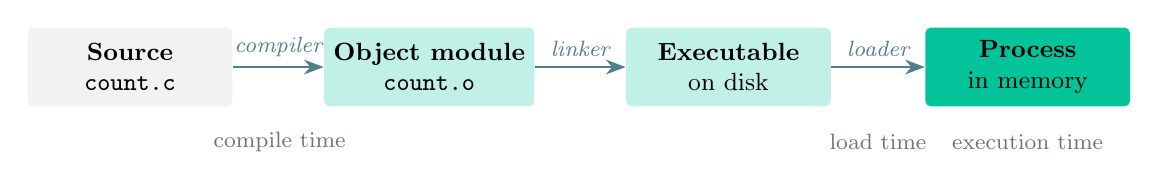
\begin{tikzpicture}[
  st/.style={rectangle,rounded corners=2pt,minimum width=2.6cm,minimum height=1.0cm,align=center,font=\small},
  arr/.style={-{Stealth[length=2.5mm]},color=slate,thick}]
\node[st,fill=light] (src) at (0,0) {\textbf{Source}\\ \texttt{count.c}};
\node[st,fill=mint!25] (obj) at (3.8,0) {\textbf{Object module}\\ \texttt{count.o}};
\node[st,fill=mint!25] (exe) at (7.6,0) {\textbf{Executable}\\ on disk};
\node[st,fill=mint] (mem) at (11.4,0) {\textbf{Process}\\ in memory};
\draw[arr] (src) -- node[above,font=\footnotesize\itshape,text=slate]{compiler} (obj);
\draw[arr] (obj) -- node[above,font=\footnotesize\itshape,text=slate]{linker} (exe);
\draw[arr] (exe) -- node[above,font=\footnotesize\itshape,text=slate]{loader} (mem);
\node[font=\footnotesize,text=muted] at (1.9,-0.95) {compile time};
\node[font=\footnotesize,text=muted] at (9.5,-0.95) {load time};
\node[font=\footnotesize,text=muted] at (11.4,-0.95) {execution time};
\end{tikzpicture}
\caption{From source code to a running process.}
\end{figure}

\begin{description}[leftmargin=0pt,style=nextline,itemsep=0.3em]
  \item[Compile time] If it is known at compile time where the process will reside in memory, the compiler can generate \term{absolute code}. If the starting location changes, the program must be recompiled. MS-DOS \texttt{.COM} programs worked this way.
  \item[Load time] Otherwise, the compiler generates \term{relocatable code}: addresses such as ``14 bytes from the beginning of this module''. The loader converts them into absolute addresses when the program is brought into memory. After loading, the program cannot move.
  \item[Execution time] If the process may be moved during its execution, binding must be delayed until the instruction actually runs: every address is translated by hardware on every memory access. This needs special hardware, the MMU, but it is what all modern general-purpose operating systems do.
\end{description}

\subsection{Logical versus physical addresses}

An address generated by the CPU while executing a program is a \term{logical address}; with execution-time binding it is also called a \term{virtual address}. The address actually seen by the memory unit, placed on the memory bus, is a \term{physical address}. The set of all logical addresses a program may generate is its \term{logical address space}; the corresponding set of physical addresses is its \term{physical address space}.

With compile-time and load-time binding, logical and physical addresses are identical. With execution-time binding they differ, and the run-time translation is performed by a hardware device called the \term{memory-management unit} (MMU). The user program never sees physical addresses: every pointer you print with \cmd{printf("\%p")} is logical. We will prove this experimentally in Section~\ref{sec:handson}.

\subsection{The simplest MMU: a relocation register}

The simplest MMU contains one \term{relocation register}, also called the \term{base register}. Its value is added to every address generated by a user process at the moment it is sent to memory.

\begin{figure}[H]
\centering
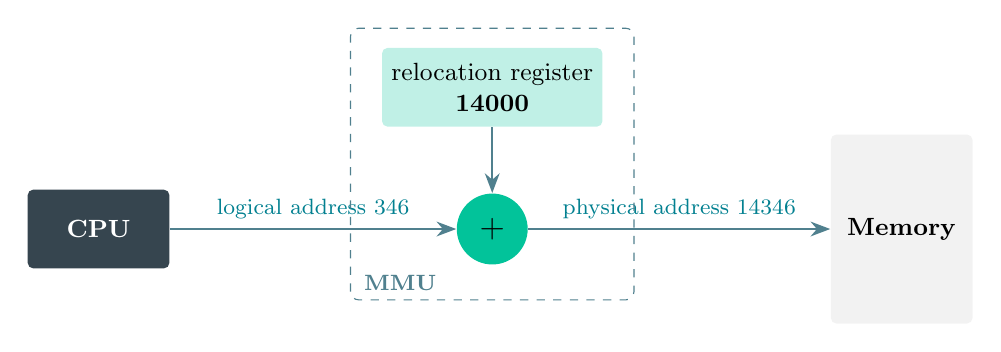
\begin{tikzpicture}[
  b/.style={rectangle,rounded corners=2pt,minimum height=1.0cm,align=center,font=\small},
  arr/.style={-{Stealth[length=2.5mm]},color=slate,thick}]
\node[b,fill=charcoal,text=white,minimum width=1.8cm] (cpu) at (0,0) {\textbf{CPU}};
\node[circle,fill=mint,minimum size=0.9cm,font=\large\bfseries] (add) at (5,0) {$+$};
\node[b,fill=mint!25,minimum width=2.8cm] (rel) at (5,1.8) {relocation register\\ \textbf{14000}};
\node[b,fill=light,minimum width=1.8cm,minimum height=2.4cm] (mem) at (10.2,0) {\textbf{Memory}};
\draw[arr] (cpu) -- node[above,font=\footnotesize,text=mintdeep]{logical address $346$} (add);
\draw[arr] (rel) -- (add);
\draw[arr] (add) -- node[above,font=\footnotesize,text=mintdeep]{physical address $14346$} (mem);
\draw[dashed,slate,rounded corners=3pt] (3.2,-0.9) rectangle (6.8,2.55);
\node[font=\footnotesize\bfseries,text=slate,anchor=south west] at (3.25,-0.9) {MMU};
\end{tikzpicture}
\caption{Dynamic relocation using a relocation register.}
\end{figure}

The program believes that it occupies addresses $0$ to $2999$. The OS has loaded it at physical address $14000$ and written $14000$ into the relocation register. When the CPU executes ``load the word at address $346$'', the MMU sends $14000 + 346 = 14346$ to memory. To move the process, the OS copies its bytes elsewhere and changes one register. Loading the relocation register is a \emph{privileged} instruction (Week~2): only the kernel may change it.

\subsection{Protection with base and limit registers}

Relocation alone does not protect anything: a program could use a very large logical address and reach another process. A second register, the \term{limit register}, holds the size of the logical address space. The MMU first checks the logical address against the limit, and only then adds the base:
\[
\text{if } 0 \le a_{\text{log}} < \text{limit:}\quad a_{\text{phys}} = \text{base} + a_{\text{log}};
\qquad \text{otherwise: trap to the OS (addressing error).}
\]

\begin{figure}[H]
\centering
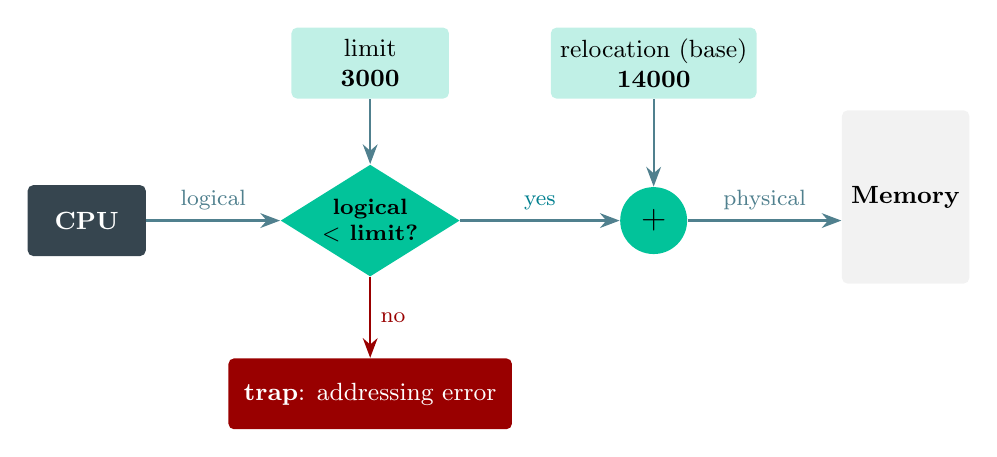
\begin{tikzpicture}[
  b/.style={rectangle,rounded corners=2pt,minimum height=0.9cm,align=center,font=\small},
  arr/.style={-{Stealth[length=2.5mm]},color=slate,thick}]
\node[b,fill=charcoal,text=white,minimum width=1.5cm] (cpu) at (0,0) {\textbf{CPU}};
\node[diamond,aspect=1.6,fill=mint,inner sep=1pt,font=\footnotesize\bfseries,align=center] (chk) at (3.6,0) {logical\\$<$ limit?};
\node[b,fill=mint!25,minimum width=2.0cm] (lim) at (3.6,2.0) {limit\\ \textbf{3000}};
\node[circle,fill=mint,minimum size=0.85cm,font=\large\bfseries] (add) at (7.2,0) {$+$};
\node[b,fill=mint!25,minimum width=2.4cm] (base) at (7.2,2.0) {relocation (base)\\ \textbf{14000}};
\node[b,fill=light,minimum width=1.6cm,minimum height=2.2cm] (mem) at (10.4,0.3) {\textbf{Memory}};
\node[b,fill=red!60!black,text=white,minimum width=3.6cm] (trap) at (3.6,-2.2) {\textbf{trap}: addressing error};
\draw[arr] (cpu) -- node[above,font=\footnotesize]{logical} (chk);
\draw[arr] (lim) -- (chk);
\draw[arr] (chk) -- node[above,font=\footnotesize,text=mintdeep]{yes} (add);
\draw[arr] (base) -- (add);
\draw[arr] (add) -- node[above,font=\footnotesize]{physical} (mem.west|-add);
\draw[arr,red!60!black] (chk) -- node[right,font=\footnotesize]{no} (trap);
\end{tikzpicture}
\caption{Hardware address protection with base and limit registers.}
\end{figure}

Because the check happens in hardware, on every access, in parallel with the addition, protection costs essentially no time. When the check fails, the CPU raises a trap (a software-generated interrupt, Week~2); the OS normally terminates the process. On Linux you see this as the message \emph{Segmentation fault (core dumped)}; today it is produced by the paging hardware (Section~\ref{sec:protbits}), but the idea is the same.

\begin{example}[Base and limit in decimal and in hexadecimal]
\textbf{Decimal.} $\text{base} = 14000$, $\text{limit} = 3000$.
\begin{itemize}
  \item $a = 346$: $346 < 3000$, so $a_{\text{phys}} = 14000 + 346 = 14346$.
  \item $a = 2999$: $2999 < 3000$, so $a_{\text{phys}} = 16999$, the last byte the process may use.
  \item $a = 3500$: $3500 \ge 3000$: \textbf{trap}.
\end{itemize}
The process owns exactly the physical range $[\text{base},\ \text{base}+\text{limit}) = [14000,\ 17000)$.

\textbf{Hexadecimal.} $\text{base} = \texttt{0x4000}$ ($=16384$), $\text{limit} = \texttt{0x1000}$ ($=4096$).
\begin{itemize}
  \item $a = \texttt{0x02A4}$ ($=676$): $\texttt{0x02A4} < \texttt{0x1000}$, so $a_{\text{phys}} = \texttt{0x4000} + \texttt{0x02A4} = \texttt{0x42A4}$. Check in decimal: $16384 + 676 = 17060 = \texttt{0x42A4}$.
  \item $a = \texttt{0x1200}$: $\texttt{0x1200} \ge \texttt{0x1000}$: \textbf{trap}.
\end{itemize}
Because the low three hex digits of the base are zero, the addition simply writes the offset into those digits. The legal physical range is \texttt{0x4000}--\texttt{0x4FFF}.
\end{example}

\begin{histnote}[Base and limit in real machines]
The CDC~6600 supercomputer (1964) protected each job with two registers called RA (reference address) and FL (field length), exactly the base/limit pair described here. The IBM~System/360 used a different scheme (4-bit storage keys on 2~KB blocks). On today's PCs, the base/limit idea survives inside the segment descriptors of x86 processors (Section~\ref{sec:x86}).
\end{histnote}

% =====================================================================
\section{Swapping}

If there is not enough RAM for all processes, the OS can temporarily move a process out of memory to a \term{backing store} (a fast disk or SSD) and bring it back later. This is \term{swapping}. The swapped-out process cannot run until it is swapped in again; if execution-time binding is used, it may come back to a different place in RAM.

\begin{figure}[H]
\centering
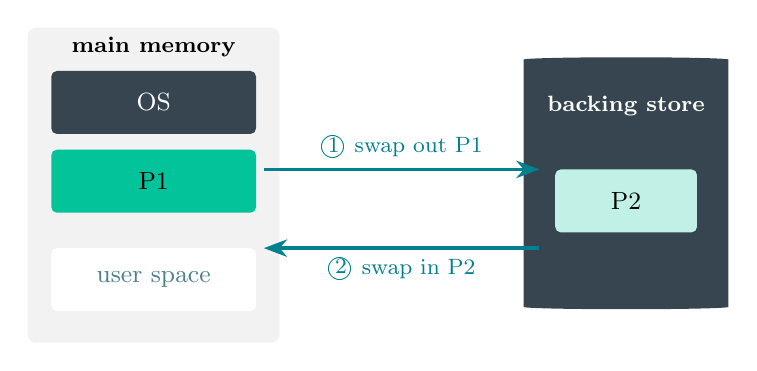
\begin{tikzpicture}[b/.style={rectangle,rounded corners=2pt,minimum width=2.6cm,minimum height=0.8cm,align=center,font=\small}]
\fill[light,rounded corners=3pt] (-1.6,-2.6) rectangle (1.6,1.4);
\node[font=\footnotesize\bfseries] at (0,1.15) {main memory};
\node[b,fill=charcoal,text=white] at (0,0.45) {OS};
\node[b,fill=mint] (p1) at (0,-0.55) {P1};
\node[b,fill=white,text=slate] at (0,-1.8) {user space};
\node[cylinder,shape border rotate=90,aspect=0.25,fill=charcoal,text=white,minimum width=2.6cm,minimum height=3.2cm,align=center,font=\small] (disk) at (6,-0.6) {};
\node[font=\footnotesize\bfseries,text=white] at (6,0.4) {backing store};
\node[b,fill=mint!25,minimum width=1.8cm] (p2) at (6,-0.8) {P2};
\draw[-{Stealth},very thick,mintdeep] (1.4,-0.4) -- node[above,font=\footnotesize]{\textcircled{1} swap out P1} (4.9,-0.4);
\draw[-{Stealth},very thick,mintdeep] (4.9,-1.4) -- node[below,font=\footnotesize]{\textcircled{2} swap in P2} (1.4,-1.4);
\end{tikzpicture}
\caption{Swapping two processes using a disk as a backing store.}
\end{figure}

The cost of swapping is dominated by the \emph{transfer time}, which is proportional to the amount of memory moved.

\begin{example}[How long does a swap take?]
A process occupies $100$~MB; the backing store transfers $50$~MB/s. Swapping it out takes
\[
t_{\text{out}} = \frac{100\ \text{MB}}{50\ \text{MB/s}} = 2\ \text{s},
\]
and swapping another process of the same size in takes another $2$~s: about $4$~s in total, ignoring disk latency. Compare with a Round-Robin time quantum of $10$~ms (Week~5): one swap costs as much as $4\ \text{s} / 10\ \text{ms} = 400$ quanta.

By contrast, moving a single $4$~KB page at the same rate takes $4096\ \text{B} / (50\times10^{6}\ \text{B/s}) \approx 82\ \mu\text{s}$.
\end{example}

For this reason, standard whole-process swapping is no longer used by general-purpose systems except, at most, in emergencies. Linux, Windows and macOS instead swap individual \emph{pages} (Section~\ref{sec:paging}); the details, demand paging and page replacement, are the subject of Week~7. Mobile systems (iOS, Android) usually do not swap at all: when memory runs low they ask background apps to save their state and then terminate them.

% =====================================================================
\section{Contiguous Memory Allocation}
\label{sec:contig}

In \term{contiguous allocation}, each process occupies a single contiguous block of physical memory. With base and limit registers this is the natural scheme: one pair of numbers describes the whole process.

\subsection{Variable partitions and the hole list}

In the \term{variable-partition} scheme the OS gives each process a block of exactly the size it needs. Initially all user memory is one large free block. As processes arrive and terminate, memory becomes a patchwork of allocated blocks and free blocks called \term{holes}. The OS keeps a list of the holes. When a process arrives, the OS searches for a hole that is large enough, allocates what is needed and leaves the rest as a smaller hole. When a process terminates, its block becomes a hole, which is merged with any neighbouring holes.

Throughout this section we use one example. Memory has $2800$~KB (a toy size, so that the numbers stay readable); the OS occupies the first $300$~KB, five processes P1--P5 are resident, and there are five holes:

\begin{figure}[H]
\centering
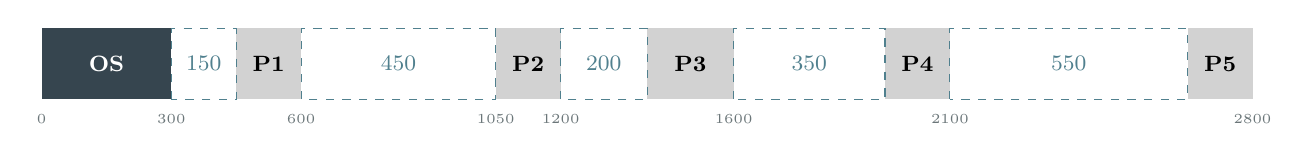
\begin{tikzpicture}[x=0.0055cm]
\fill[charcoal] (0,0) rectangle (300,0.9);
\node[font=\footnotesize\bfseries,text=white] at (150,0.45) {OS};
\foreach \a/\b/\t in {450/600/P1, 1050/1200/P2, 1400/1600/P3, 1950/2100/P4, 2650/2800/P5} {
  \fill[gray!35] (\a,0) rectangle (\b,0.9);
  \node[font=\footnotesize\bfseries] at ({(\a+\b)/2},0.45) {\t};
}
\foreach \a/\s in {300/150, 600/450, 1200/200, 1600/350, 2100/550} {
  \draw[slate,dashed] (\a,0) rectangle ({\a+\s},0.9);
  \node[font=\footnotesize,text=slate] at ({\a+\s/2},0.45) {\s};
}
\foreach \a in {0,300,600,1050,1200,1600,2100,2800} \node[font=\tiny,text=muted] at (\a,-0.25) {\a};
\end{tikzpicture}
\caption{The running example: hole sizes in KB, addresses in KB below the bar.}
\end{figure}

The hole list, as (start, size) pairs in address order, is
\[
(300,150),\ (600,450),\ (1200,200),\ (1600,350),\ (2100,550),\qquad \text{total free} = 1700\ \text{KB}.
\]

\subsection{Placement algorithms: first-fit, best-fit, worst-fit}

Which hole should a new process get? The three classical strategies are:
\begin{description}[leftmargin=0pt,style=nextline,itemsep=0.3em]
  \item[First-fit] Allocate the \emph{first} hole that is big enough. Searching can stop as soon as one is found (from the start of the list, or from where the last search ended, a variant called next-fit).
  \item[Best-fit] Allocate the \emph{smallest} hole that is big enough. The whole list must be searched, unless it is kept sorted by size. Produces the smallest leftover hole.
  \item[Worst-fit] Allocate the \emph{largest} hole. Also needs a full search. The idea is that the leftover remains large enough to be useful.
\end{description}

\begin{example}[Four requests, three strategies]
Processes arrive in the order A $=220$~KB, B $=400$~KB, C $=130$~KB, D $=430$~KB. Each request is carved from the beginning of the chosen hole.

\textbf{Request A (220 KB).} Holes large enough: $450$, $350$, $550$. First-fit takes the first in address order, $450@600$; best-fit the smallest, $350@1600$; worst-fit the largest, $550@2100$.

Continuing in the same way:
\begin{center}
\renewcommand{\arraystretch}{1.25}
\begin{tabular}{@{}lccc@{}}
\toprule
\textbf{Request} & \textbf{First-fit} & \textbf{Best-fit} & \textbf{Worst-fit} \\
\midrule
A = 220 & $450@600$ $\to$ leaves $230$ & $350@1600$ $\to$ leaves $130$ & $550@2100$ $\to$ leaves $330$ \\
B = 400 & $550@2100$ $\to$ leaves $150$ & $450@600$ $\to$ leaves $50$ & $450@600$ $\to$ leaves $50$ \\
C = 130 & $150@300$ $\to$ leaves $20$ & $130@1820$ $\to$ leaves $0$ & $350@1600$ $\to$ leaves $220$ \\
D = 430 & \textcolor{red!60!black}{must wait} & $550@2100$ $\to$ leaves $120$ & \textcolor{red!60!black}{must wait} \\
\bottomrule
\end{tabular}
\end{center}
With first-fit, $950$~KB are free when D arrives, but the largest hole is only $350$~KB; with worst-fit the largest is $330$~KB. Only best-fit places all four processes in this example.
\end{example}

The table was verified with a small Python script, \texttt{code/fit.py}. Its heart is the function that chooses a hole; the rest of the script just loops over the requests and prints the result:

\lstinputlisting[language=Python,caption={},firstline=16,lastline=25,firstnumber=16]{../code/fit.py}

\begin{lstlisting}[style=term]
$ python3 fit.py
\end{lstlisting}
\vspace{-0.9em}
\lstinputlisting[style=term]{../code/out_fit.txt}

One example proves nothing in general: best-fit tends to leave many tiny, useless holes (here $50$~KB and, in other sequences, holes of a few bytes). Simulations reported by Silberschatz show that first-fit and best-fit are better than worst-fit in both time and storage utilisation; neither first-fit nor best-fit is clearly better in storage use, but first-fit is generally faster.

\subsection{Fragmentation}

\paragraph{External fragmentation.} Enough total memory exists to satisfy a request, but it is not contiguous: it is split into many small holes. In the first-fit run, $950$~KB were free but D ($430$~KB) could not be loaded. External fragmentation is typical of every scheme that hands out variable-size blocks (variable partitions, segmentation).

\begin{keyidea}[The 50-percent rule]
Statistical analysis of first-fit (quoted by Silberschatz, after Knuth) shows that, even with some optimisation, if $N$ blocks are allocated, another $0.5N$ blocks are lost to fragmentation. The fraction of memory that may be unusable is then
\[
\frac{0.5N}{N + 0.5N} = \frac{1}{3}.
\]
\end{keyidea}

\paragraph{Internal fragmentation.} Memory allocated to a process but not used by it: waste \emph{inside} a block. It arises whenever memory is handed out in fixed-size units. Suppose a hole of $18\,464$ bytes is available and a process requests $18\,462$ bytes. Keeping a $2$-byte hole in the list would cost more (list entry) than the hole itself, so the allocator gives away all $18\,464$ bytes; $2$ bytes are internally fragmented. Internal fragmentation is typical of fixed partitions and of paging.

\subsection{Compaction}

One cure for external fragmentation is \term{compaction}: shuffle the memory contents so that all free memory is placed together in one large block. In our first-fit result the blocks OS, C, P1, A, P2, P3, P4, B, P5 occupy $1850$~KB; moved to the low end of memory they leave a single hole of $2800 - 1850 = 950$~KB, and D fits (leaving $520$~KB).

Compaction is possible only if relocation is dynamic (execution-time binding): the OS moves the bytes and updates the base register. It is also expensive: in the worst case all of memory is copied, the affected processes must be stopped, and a process doing I/O into a buffer cannot be moved while the device writes into that buffer. A better cure is to allow a process's memory to be \emph{non-contiguous}. That is the idea of paging.

% =====================================================================
\section{Paging}
\label{sec:paging}

\subsection{Pages and frames}

\term{Paging} avoids external fragmentation completely. Physical memory is divided into fixed-size blocks called \term{frames}; logical memory is divided into blocks of the same size called \term{pages}. When a process is loaded, its pages are placed into \emph{any} available frames. A per-process \term{page table} records, for each page, the frame that holds it. The OS keeps a list of free frames.

\begin{figure}[H]
\centering
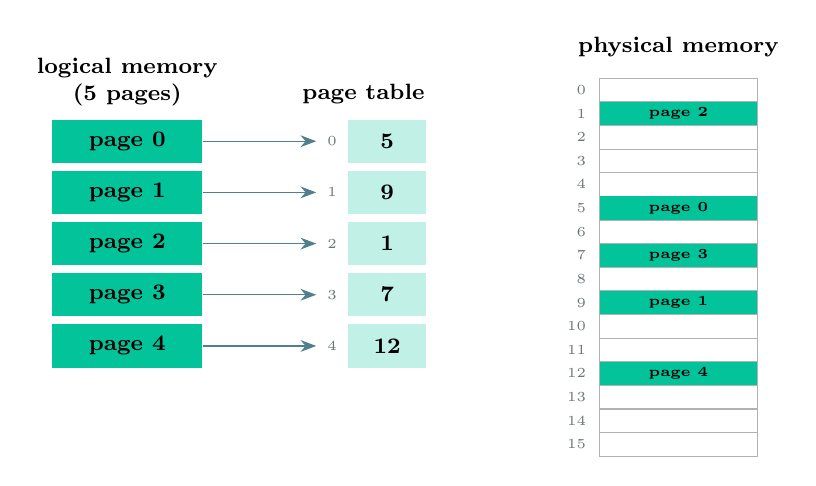
\begin{tikzpicture}[
  pg/.style={rectangle,fill=mint,minimum width=1.9cm,minimum height=0.55cm,font=\footnotesize\bfseries},
  pt/.style={rectangle,fill=mint!25,minimum width=1.0cm,minimum height=0.55cm,font=\footnotesize\bfseries},
  arr/.style={-{Stealth[length=2mm]},color=slate}]
\node[font=\footnotesize\bfseries,align=center] at (0,0.75) {logical memory\\(5 pages)};
\foreach \i/\f in {0/5,1/9,2/1,3/7,4/12} {
  \node[pg] (p\i) at (0,-\i*0.65) {page \i};
  \node[font=\tiny,text=muted] at (2.6,-\i*0.65) {\i};
  \node[pt] (t\i) at (3.3,-\i*0.65) {\f};
  \draw[arr] (p\i.east) -- (2.4,-\i*0.65);
}
\node[font=\footnotesize\bfseries] at (3.0,0.6) {page table};
\node[font=\footnotesize\bfseries] at (7.0,1.2) {physical memory};
\foreach \f in {0,...,15} {
  \pgfmathsetmacro{\yy}{0.8-\f*0.3}
  \draw[gray!60,fill=white] (6.0,\yy) rectangle (8.0,\yy-0.3);
  \node[font=\tiny,text=muted,anchor=east] at (5.95,\yy-0.15) {\f};
}
\foreach \i/\f in {0/5,1/9,2/1,3/7,4/12} {
  \pgfmathsetmacro{\yy}{0.8-\f*0.3}
  \fill[mint] (6.0,\yy) rectangle (8.0,\yy-0.3);
  \node[font=\tiny\bfseries] at (7.0,\yy-0.15) {page \i};
}
\end{tikzpicture}
\caption{Paging: five pages of a process scattered over sixteen frames. This page table is used in all examples below and in \texttt{page\_split.c}.}
\end{figure}

The page size is defined by the hardware and is always a power of~$2$, typically $4$~KB (Linux on x86-64; \cmd{getconf PAGESIZE} prints $4096$), sometimes $16$~KB (Apple silicon) or larger.

\subsection{Splitting an address into page number and offset}

If the logical address space has $2^{m}$ bytes ($m$-bit addresses) and the page size is $2^{n}$ bytes, then the high-order $m-n$ bits of a logical address give the \term{page number} $p$, and the low-order $n$ bits give the \term{page offset} $d$:
\begin{center}

\begin{tikzpicture}
\node[rectangle,fill=mint,minimum width=5.5cm,minimum height=0.8cm,align=center,font=\small] (p) {page number $p$\\ $m-n$ bits};
\node[rectangle,fill=charcoal,text=white,minimum width=4cm,minimum height=0.8cm,align=center,font=\small,right=0pt of p] {page offset $d$\\ $n$ bits};
\end{tikzpicture}
\end{center}
\[
p = \left\lfloor \frac{a}{2^{n}} \right\rfloor = a \gg n, \qquad
d = a \bmod 2^{n} = a \mathbin{\&} (2^{n}-1), \qquad
a_{\text{phys}} = f \cdot 2^{n} + d,
\]
where $f$ is the frame number found in entry $p$ of the page table. Because the page size is a power of~$2$, no division is needed: the hardware simply uses the upper bits as an index into the page table and copies the lower bits unchanged. For example, with $16$-bit addresses and $4$~KB pages ($n=12$), $p$ has $4$ bits and the address space has $2^{4}=16$ pages; with $32$-bit addresses, $p$ has $20$ bits ($2^{20}$ pages).

A useful shortcut: one hexadecimal digit is exactly $4$ bits, so with $4$~KB pages the offset is the last three hex digits of the address.

\begin{example}[Translating logical address \texttt{0x3A7F}]
$16$-bit addresses, $4$~KB pages, the page table of the figure above (page $0\to5$, $1\to9$, $2\to1$, $3\to7$, $4\to12$).

In binary, $\texttt{0x3A7F} = \underbrace{0011}_{p}\ \underbrace{1010\ 0111\ 1111}_{d}$, so $p = 3$ and $d = \texttt{0xA7F}$.

In decimal: $\texttt{0x3A7F} = 14975$; $p = \lfloor 14975/4096 \rfloor = 3$, $d = 14975 - 3\cdot4096 = 2687 = \texttt{0xA7F}$.

The page table gives frame $f = 7$, hence
\[
a_{\text{phys}} = 7 \times 4096 + 2687 = 28672 + 2687 = 31359 = \texttt{0x7A7F}.
\]
In hex, just replace the page digit $3$ by the frame digit $7$. Similarly, $\texttt{0x1234}$ has $p=1$, $d=\texttt{0x234}$, frame $9$, physical $\texttt{0x9234} = 37428$; and $\texttt{0x5000}$ has $p = 5$, which is not part of the process: trap.
\end{example}

\begin{figure}[H]
\centering
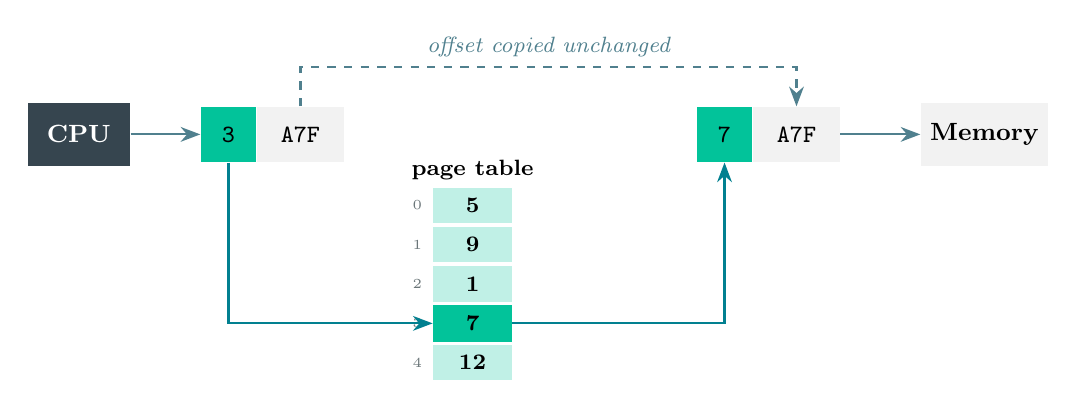
\begin{tikzpicture}[
  f/.style={rectangle,minimum height=0.7cm,font=\small\ttfamily},
  arr/.style={-{Stealth[length=2.5mm]},color=slate,thick}]
\node[rectangle,fill=charcoal,text=white,minimum width=1.3cm,minimum height=0.8cm,font=\small\bfseries] (cpu) at (0,0) {CPU};
\node[f,fill=mint,minimum width=0.7cm] (p) at (1.9,0) {3};
\node[f,fill=light,minimum width=1.1cm,right=0pt of p] (d) {A7F};
\node[f,fill=mint,minimum width=0.7cm] (f) at (8.2,0) {7};
\node[f,fill=light,minimum width=1.1cm,right=0pt of f] (d2) {A7F};
\node[rectangle,fill=light,minimum width=1.6cm,minimum height=0.8cm,font=\small\bfseries] (mem) at (11.5,0) {Memory};
\draw[arr] (cpu) -- (p);
\draw[arr] (d2) -- (mem);
\foreach \i/\v in {0/5,1/9,2/1,3/7,4/12} {
  \node[rectangle,fill=mint!25,minimum width=1.0cm,minimum height=0.45cm,font=\footnotesize\bfseries] (r\i) at (5.0,-0.9-\i*0.5) {\v};
  \node[font=\tiny,text=muted] at (4.3,-0.9-\i*0.5) {\i};
}
\node[font=\footnotesize\bfseries] at (5.0,-0.45) {page table};
\fill[mint] ($(r3.south west)$) rectangle ($(r3.north east)$); \node[font=\footnotesize\bfseries] at (r3) {7};
\draw[arr,mintdeep] (p.south) |- (r3.west);
\draw[arr,mintdeep] (r3.east) -| (f.south);
\draw[arr,dashed] (d.north) -- ++(0,0.5) -| node[pos=0.25,above,font=\footnotesize\itshape]{offset copied unchanged} (d2.north);
\end{tikzpicture}
\caption{Paging hardware translating \texttt{0x3A7F} to \texttt{0x7A7F}.}
\end{figure}

\subsection{Internal fragmentation in paging}

Paging has no external fragmentation: any free frame can hold any page. But memory is handed out in whole frames, so the last frame of a process is usually not full.

\begin{example}[A 10,000-byte process]
With $4096$-byte pages: $10\,000 = 2 \times 4096 + 1808$. The process needs $3$ frames; the third holds only $1808$ bytes, so $4096 - 1808 = 2288$ bytes are lost to internal fragmentation.
\end{example}

In the worst case a process needs $n$ pages plus one byte, wasting almost a whole frame. If process sizes are independent of the page size, the last page is on average half full: the expected internal fragmentation is \textbf{half a page per process}. This argues for small pages; but smaller pages mean more pages, larger page tables and less efficient disk I/O. Page sizes have grown over time. Linux on x86-64 uses $4$~KB pages normally, plus \emph{huge pages} of $2$~MB or $1$~GB for programs with very large memory needs (our test machine reports \texttt{Hugepagesize: 2048 kB} in \texttt{/proc/meminfo}).

\subsection{How large is a page table?}

A page table has one entry per page of the logical address space.

\begin{example}[Page-table size for a 32-bit address space]
$32$-bit logical addresses, $4$~KB pages, $4$-byte page-table entries:
\[
\text{entries} = \frac{2^{32}}{2^{12}} = 2^{20} = 1\,048\,576,
\qquad
\text{size} = 2^{20} \times 4\ \text{B} = 2^{22}\ \text{B} = 4\ \text{MB}
\]
\emph{per process}. With $100$ processes that is $400$~MB of page tables, most of which would describe unused parts of the address space. For $64$-bit systems the problem is far worse: a flat table for a $48$-bit address space with $8$-byte entries would need $2^{36} \times 8\ \text{B} = 512$~GB.
\end{example}

The solution, which we only outline, is the \term{multi-level} (hierarchical) page table: the page table is itself paged. In a two-level scheme for $32$-bit addresses, the $20$-bit page number is split into $p_1$ ($10$ bits) indexing an outer table of $2^{10}$ entries (exactly one $4$~KB page) and $p_2$ ($10$ bits) indexing an inner table; inner tables exist only for the parts of the address space that are actually used. x86-64 uses four levels ($9+9+9+9$ bits of page number plus a $12$-bit offset $=48$ bits); recent processors support a fifth level ($57$-bit addresses). Each table at every level fits in exactly one $4$~KB page ($2^{9}$ entries of $8$ bytes).

\subsection{The translation look-aside buffer (TLB)}

The page table is kept in main memory, and a register (on x86, \texttt{CR3}) points to it. Then every data access needs \emph{two} memory accesses: one for the page-table entry, one for the data itself. Paging would halve the speed of memory. The standard solution is a small, fast hardware cache inside the MMU, the \term{translation look-aside buffer} (TLB). Each TLB entry holds a (page number, frame number) pair; all entries are searched in parallel (associative memory). TLBs typically have between $32$ and about $1536$ entries.

\begin{figure}[H]
\centering
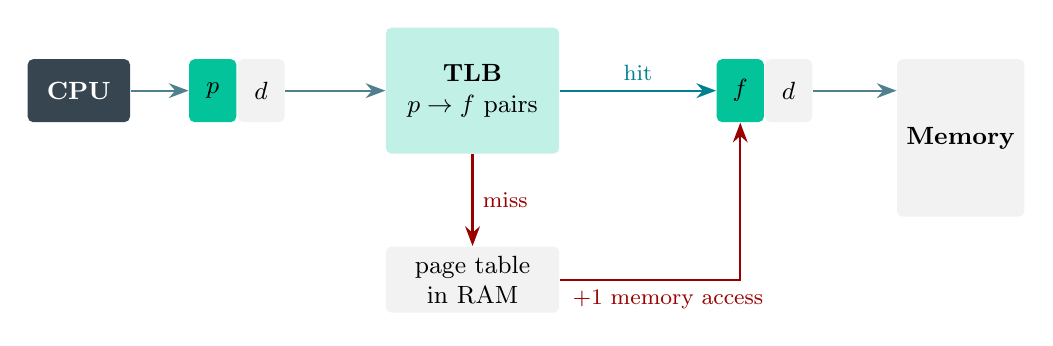
\begin{tikzpicture}[
  b/.style={rectangle,rounded corners=2pt,minimum height=0.8cm,align=center,font=\small},
  arr/.style={-{Stealth[length=2.5mm]},color=slate,thick}]
\node[b,fill=charcoal,text=white,minimum width=1.3cm] (cpu) at (0,0) {\textbf{CPU}};
\node[b,fill=mint,minimum width=0.6cm] (p) at (1.7,0) {$p$};
\node[b,fill=light,minimum width=0.6cm,right=0pt of p] (d) {$d$};
\node[b,fill=mint!25,minimum width=2.2cm,minimum height=1.6cm] (tlb) at (5.0,0) {\textbf{TLB}\\ $p \to f$ pairs};
\node[b,fill=light,minimum width=2.2cm] (pt) at (5.0,-2.4) {page table\\ in RAM};
\node[b,fill=mint,minimum width=0.6cm] (f) at (8.4,0) {$f$};
\node[b,fill=light,minimum width=0.6cm,right=0pt of f] (d2) {$d$};
\node[b,fill=light,minimum width=1.4cm,minimum height=2.0cm] (mem) at (11.2,-0.6) {\textbf{Memory}};
\draw[arr] (cpu) -- (p);
\draw[arr] (d.east) -- (tlb.west);
\draw[arr,mintdeep] (tlb) -- node[above,font=\footnotesize]{hit} (f);
\draw[arr,red!60!black] (tlb) -- node[right,font=\footnotesize]{miss} (pt);
\draw[arr,red!60!black] (pt.east) -| node[pos=0.3,below,font=\footnotesize]{$+1$ memory access} (f.south);
\draw[arr] (d2.east) -- (mem.west|-d2);
\end{tikzpicture}
\caption{Paging hardware with a TLB.}
\end{figure}

On a \emph{TLB hit} the frame number is available almost immediately. On a \emph{TLB miss} the page-table entry must be read from memory (by hardware on x86, by the OS on some other architectures), and it is then stored in the TLB, possibly replacing an older entry. Because programs show \emph{locality} (loops execute the same code, arrays are traversed sequentially, the stack is used near its top), hit ratios above $99\%$ are common. On a context switch the TLB entries of the old process must be flushed, or tagged with an address-space identifier (ASID) so that they cannot be used by the new process.

\subsubsection{Effective access time}

Let $\alpha$ be the \term{hit ratio} (the fraction of accesses that find their page number in the TLB), $t_{m}$ the time of one memory access and $t_{\text{TLB}}$ the time of one TLB lookup.

\begin{keyidea}[Convention used in this course]
We count the TLB lookup on every access, and a miss costs one extra memory access:
\[
\text{EAT} = \alpha\,(t_{\text{TLB}} + t_{m}) + (1-\alpha)\,(t_{\text{TLB}} + 2t_{m}) = t_{\text{TLB}} + (2-\alpha)\,t_{m}.
\]
\end{keyidea}

\begin{example}[Effective access time]
Take $t_{\text{TLB}} = 20$~ns and $t_{m} = 100$~ns.
\begin{align*}
\alpha = 0.80:&\quad \text{EAT} = 0.80 \times 120 + 0.20 \times 220 = 96 + 44 = 140\ \text{ns} &&(40\%\ \text{slower than } t_m),\\
\alpha = 0.98:&\quad \text{EAT} = 0.98 \times 120 + 0.02 \times 220 = 117.6 + 4.4 = 122\ \text{ns} &&(22\%\ \text{slower}).
\end{align*}
Without any TLB, every access costs $2t_{m} = 200$~ns. Check with the short form: $20 + (2-0.98)\times100 = 122$~ns.
\end{example}

\paragraph{The modern simplification.} On current CPUs the TLB lookup takes about one clock cycle and is overlapped with other work, so the 10th edition of Silberschatz ignores it ($t_{\text{TLB}}\approx 0$):
\[
\text{EAT} = \alpha\,t_{m} + (1-\alpha)\,2t_{m}.
\]
With $t_{m} = 100$~ns this gives $120$~ns for $\alpha = 0.80$ and $101$~ns for $\alpha = 0.99$ (Silberschatz uses $t_{m}=10$~ns: $12$~ns and $10.1$~ns). In an exam, always state which convention you use. All numbers in this section are checked by \texttt{code/verify.py}.

\subsection{Protection bits and the valid--invalid bit}
\label{sec:protbits}

A page-table entry contains more than a frame number. Protection bits stored in each entry are checked by the MMU on every access, in parallel with the translation:
\begin{itemize}
  \item A \term{valid--invalid bit}. \emph{Valid} means the page belongs to the process's logical address space; \emph{invalid} means it does not, and any access traps to the OS.
  \item \textbf{Read / write / execute} permissions. A write to a read-only page, or an attempt to execute instructions from a page marked no-execute (the NX bit of x86-64), also traps.
\end{itemize}

\begin{center}
\renewcommand{\arraystretch}{1.2}
\begin{tabular}{@{}ccccl@{}}
\toprule
\textbf{Page} & \textbf{Frame} & \textbf{Valid} & \textbf{Permissions} & \textbf{Contents} \\
\midrule
0 & 5 & v & \texttt{r-x} & code \\
1 & 9 & v & \texttt{r-x} & code \\
2 & 1 & v & \texttt{rw-} & data \\
3 & 7 & v & \texttt{rw-} & heap \\
4 & 12 & v & \texttt{rw-} & stack \\
5--15 & --- & i & --- & not part of the process \\
\bottomrule
\end{tabular}
\end{center}

With this table, logical address \texttt{0x5000} (page $5$) traps because the page is invalid, and a write into page $0$ traps because code pages are read-only. The same letters \texttt{r}, \texttt{w}, \texttt{x} appear in \texttt{/proc/self/maps} (Section~\ref{sec:handson}). Next week the valid bit will get a second use: a page may belong to the process but currently not be in RAM (a \emph{page fault}, Week~7).

\subsection{Shared pages}

Paging makes it easy to share code. If code is \term{reentrant} (it never modifies itself), one copy in physical memory can be mapped into the page tables of many processes. A typical example is the C library \texttt{libc}: every process on a Linux machine uses it, but its code pages are in RAM only once. Only each process's private data pages are separate.

\begin{figure}[H]
\centering
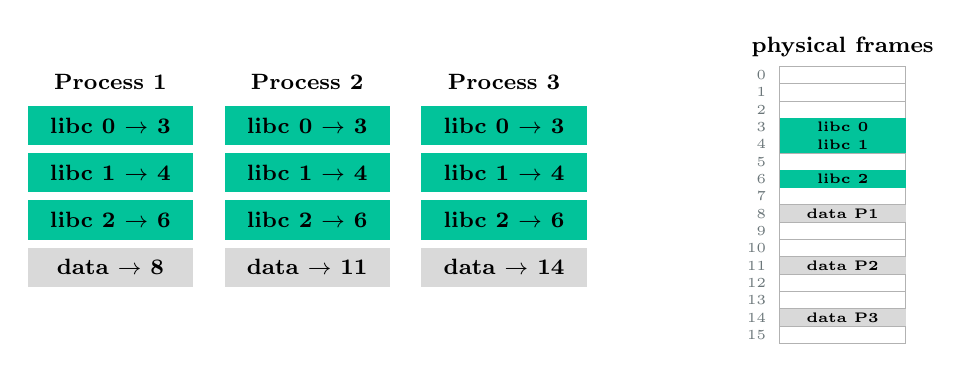
\begin{tikzpicture}[
  pg/.style={rectangle,minimum width=2.1cm,minimum height=0.5cm,font=\footnotesize\bfseries}]
\foreach \k/\d in {0/8,1/11,2/14} {
  \node[font=\footnotesize\bfseries] at (\k*2.5,0.55) {Process \the\numexpr\k+1\relax};
  \node[pg,fill=mint] at (\k*2.5,0) {libc 0 $\to$ 3};
  \node[pg,fill=mint] at (\k*2.5,-0.6) {libc 1 $\to$ 4};
  \node[pg,fill=mint] at (\k*2.5,-1.2) {libc 2 $\to$ 6};
  \node[pg,fill=gray!30] at (\k*2.5,-1.8) {data $\to$ \d};
}
\node[font=\footnotesize\bfseries] at (9.3,1.0) {physical frames};
\foreach \f in {0,...,15} {
  \pgfmathsetmacro{\yy}{0.75-\f*0.22}
  \draw[gray!60] (8.5,\yy) rectangle (10.1,\yy-0.22);
  \node[font=\tiny,text=muted,anchor=east] at (8.45,\yy-0.11) {\f};
}
\foreach \f/\t/\c in {3/libc 0/mint,4/libc 1/mint,6/libc 2/mint,8/data P1/gray!30,11/data P2/gray!30,14/data P3/gray!30} {
  \pgfmathsetmacro{\yy}{0.75-\f*0.22}
  \fill[\c] (8.5,\yy) rectangle (10.1,\yy-0.22);
  \node[font=\tiny\bfseries] at (9.3,\yy-0.11) {\t};
}
\end{tikzpicture}
\caption{Three processes share the three code pages of the C library; only their data pages are private.}
\end{figure}

With $40$ processes and a $2$~MB library, sharing saves $39 \times 2\ \text{MB} = 78$~MB. Shared pages are marked read-only so that no process can modify the common copy. The same mechanism lets \cmd{fork()} start by sharing \emph{all} pages between parent and child, copying a page only when one of them writes to it (\emph{copy-on-write}, Week~7).

% =====================================================================
\section{Segmentation}

\subsection{The user's view of memory}

Programmers do not think of their program as a sequence of $4$~KB pages. They think of a main program, a set of functions, a stack, a symbol table, global data, and so on. Each of these is a logical unit of a different size, and within each unit locations are identified by their distance from its start (``the fifth instruction of \cmd{sqrt()}'', ``the top of the stack''). \term{Segmentation} is a memory-management scheme that supports exactly this view: the logical address space is a collection of \term{segments}, and a logical address is a pair
\[
\langle \text{segment number } s,\ \text{offset } d \rangle .
\]
The compiler creates the segments (for example: code, global variables, heap, one stack per thread, the standard C library), and the loader assigns each one a place in physical memory.

\subsection{The segment table}
\label{sec:segtable}

The mapping is done by a \term{segment table}. Each entry has a \term{segment base} (the starting physical address of the segment) and a \term{segment limit} (its length). The offset $d$ must lie between $0$ and the limit; otherwise the hardware traps:
\[
\text{if } 0 \le d < \text{limit}[s]:\quad a_{\text{phys}} = \text{base}[s] + d;\qquad\text{otherwise: trap (addressing error).}
\]
In other words: segmentation is the base--limit idea of Section~\ref{sec:mmu} with one pair of registers \emph{per segment}.

\begin{example}[Segment-table translation]
\begin{center}
\renewcommand{\arraystretch}{1.2}
\begin{tabular}{@{}clrrl@{}}
\toprule
$s$ & \textbf{Segment} & \textbf{Base} & \textbf{Limit} & \textbf{Occupies} \\
\midrule
0 & main program & 2000 & 1200 & 2000--3199 \\
1 & \texttt{sqrt()} library & 6500 & 300 & 6500--6799 \\
2 & stack & 4800 & 600 & 4800--5399 \\
3 & symbol table & 3400 & 900 & 3400--4299 \\
4 & heap / data & 5600 & 700 & 5600--6299 \\
\bottomrule
\end{tabular}
\end{center}
\begin{itemize}
  \item $\langle 2, 53\rangle$: $53 < 600$, so $a_{\text{phys}} = 4800 + 53 = 4853$.
  \item $\langle 3, 852\rangle$: $852 < 900$, so $a_{\text{phys}} = 3400 + 852 = 4252$.
  \item $\langle 1, 299\rangle$: $299 < 300$, so $a_{\text{phys}} = 6500 + 299 = 6799$, the last byte of segment~1.
  \item $\langle 0, 1222\rangle$: $1222 \ge 1200$: \textbf{trap}. The program tried to access beyond the end of its main-program segment.
\end{itemize}
\end{example}

Because segments are units with a meaning, protection and sharing can be set per meaningful unit: code read-only and shareable, stack and data read-write and private. The price is that segments have variable sizes and must each be allocated contiguously: the problems of Section~\ref{sec:contig} (placement, external fragmentation, compaction) come back.

\subsection{Paging versus segmentation}

\begin{center}
\renewcommand{\arraystretch}{1.3}
\begin{tabularx}{\linewidth}{>{\raggedright\arraybackslash}p{3.6cm} >{\raggedright\arraybackslash}X >{\raggedright\arraybackslash}X}
\toprule
 & \textbf{Paging} & \textbf{Segmentation} \\
\midrule
Unit size & fixed (e.g.\ $4$~KB), chosen by the hardware & variable, follows the program's structure \\
Visible to the programmer? & no & yes (main, stack, data, \dots) \\
Logical address & one number, split into $p \mid d$ & a pair $\langle s, d\rangle$ \\
External fragmentation & none & yes \\
Internal fragmentation & yes, on average $\tfrac12$ page per process & none \\
Protection and sharing & per page & per segment (meaningful unit) \\
Table entry & frame number and bits & base, limit and bits \\
\bottomrule
\end{tabularx}
\end{center}

\begin{histnote}[Segments made of pages]
Several historical systems combined the two schemes: the address space was divided into segments, and each segment was divided into pages. Multics (1960s, the ancestor of UNIX) worked this way, and so did the Intel 80386 (1985), whose 32-bit protected mode first translated a segmented address into a ``linear'' address and then paged it. Both mechanisms are still present in x86 processors for compatibility.
\end{histnote}

\subsection{What x86-64 Linux actually does}
\label{sec:x86}

In 64-bit mode, Intel and AMD processors essentially switch segmentation off: the code, data and stack segments are forced to base $0$ and cover the whole address space (a \emph{flat} memory model). Only the FS and GS segment registers keep a non-zero base, which Linux uses to find thread-local data. All real translation and protection is done by \textbf{paging}:
\begin{itemize}
  \item four-level page tables for $48$-bit virtual addresses ($9+9+9+9+12$ bits), or five levels ($57$ bits) on recent processors;
  \item page sizes of $4$~KB, $2$~MB and $1$~GB;
  \item one set of page tables per process; the register \texttt{CR3} holds the physical address of the top-level table, and a context switch (Week~3) reloads it.
\end{itemize}
ARM64 processors (phones, Apple M-series) have no segmentation at all. The \emph{idea} of segments lives on in software: Linux keeps, for each process, a list of memory regions (program code, data, heap, stack, each shared library), and that is exactly what \texttt{/proc/<pid>/maps} prints. The message \emph{Segmentation fault} survives as a name, although on Linux it now reports an access outside these regions or a violation of page permissions.

% =====================================================================
\section{Hands-on: Real Addresses on Linux}
\label{sec:handson}

The programs are in the \texttt{code/} folder next to these notes and compile with \cmd{gcc -Wall -O2} (or simply \cmd{make}). All output below was captured on our Linux test machine (x86-64). Because Linux randomises the position of the regions on every run (\term{ASLR}, address-space layout randomisation, a security measure), your addresses will be different, but the pattern will be the same.

\subsection{Example 1: where do my variables live?}

The helper \cmd{show\_maps()} (see the full file \texttt{code/mem\_layout.c}) prints the lines of \texttt{/proc/self/maps} that belong to the program file, the heap and the stack. The rest of the program:

\lstinputlisting[caption={},firstline=15,lastline=17,firstnumber=15]{../code/mem_layout.c}
\vspace{-0.6em}
\lstinputlisting[caption={},firstline=37,firstnumber=37]{../code/mem_layout.c}

\begin{lstlisting}[style=term]
$ ./mem_layout
text  (code)   main()      : 0x56412f3601e0
data  (global) initialised : 0x56412f363010
bss   (global) zero-filled : 0x56412f363018
heap  (malloc)             : 0x564160c6c2a0
stack (local variable)     : 0x7ffe905b48c4
page size                  : 4096 bytes

--- my regions in /proc/self/maps ---
56412f35f000-56412f360000 r--p mem_layout
56412f360000-56412f361000 r-xp mem_layout
56412f361000-56412f362000 r--p mem_layout
56412f362000-56412f363000 r--p mem_layout
56412f363000-56412f364000 rw-p mem_layout
564160c6c000-564160c8d000 rw-p [heap]
7ffe90595000-7ffe905bb000 rw-p [stack]
\end{lstlisting}

Match each address with a region: \cmd{main} ($\texttt{0x\dots3601e0}$) lies in the \texttt{r-xp} region of the program file (readable and executable, not writable: code); the two globals lie in the \texttt{rw-p} region; the \cmd{malloc} block lies in \texttt{[heap]}; the local variable lies in \texttt{[stack]}, near the top of the user address space. Every region starts and ends at a multiple of $\texttt{0x1000} = 4096$: regions consist of whole pages. The heap region has $\texttt{0x564160c8d000} - \texttt{0x564160c6c000} = \texttt{0x21000} = 135\,168$ bytes $= 33$ pages; the stack region $\texttt{0x26000} = 155\,648$ bytes $= 38$ pages.

\Needspace{10\baselineskip}
\subsection{The page size and the memory map from the shell}

\begin{lstlisting}[style=term]
$ getconf PAGESIZE
4096
$ grep Hugepagesize /proc/meminfo
Hugepagesize:       2048 kB
$ head -n 6 /proc/self/maps
559948881000-559948883000 r--p 00000000 fe:00 270606   /usr/bin/head
559948883000-559948889000 r-xp 00002000 fe:00 270606   /usr/bin/head
559948889000-55994888b000 r--p 00008000 fe:00 270606   /usr/bin/head
55994888b000-55994888c000 r--p 00009000 fe:00 270606   /usr/bin/head
55994888c000-55994888d000 rw-p 0000a000 fe:00 270606   /usr/bin/head
559970df7000-559970e18000 rw-p 00000000 00:00 0        [heap]
\end{lstlisting}

\texttt{/proc/self} always refers to the process that reads it, here \cmd{head} itself. The columns are: virtual start--end address, permissions (\texttt{r}, \texttt{w}, \texttt{x}, and \texttt{p} for private or \texttt{s} for shared), offset in the file, device, inode and file name. For example, the code region of \cmd{head} spans $\texttt{0x559948889000} - \texttt{0x559948883000} = \texttt{0x6000} = 24\,576$ bytes $= 6$ pages. (Spacing in the last column was shortened.)

\Needspace{10\baselineskip}
\subsection{Example 2: same address, different values}

\lstinputlisting[caption={},firstline=9,firstnumber=9]{../code/fork_vaddr.c}

\begin{lstlisting}[style=term]
$ ./fork_vaddr
child  (PID 1760): &x = 0x55bc4a29c010   x = 200
parent (PID 1759): &x = 0x55bc4a29c010   x = 100
\end{lstlisting}

After \cmd{fork()} the child is a copy of the parent, so both have the same layout and \cmd{\&x} is the same number in both. Yet the child changed \cmd{x} to $200$ and the parent still sees $100$. If \cmd{\&x} were a physical address this would be impossible: one byte of RAM cannot hold two different values. The address is \emph{logical}; each process has its own page table, which maps the page containing \cmd{x} to a different physical frame. (More precisely: right after \cmd{fork()} both page tables point to the same frame, marked read-only; when the child writes, the kernel copies the page and updates the child's entry. This copy-on-write technique is part of Week~7.) Run the program several times: because of ASLR the address changes from run to run, but parent and child always agree.

\Needspace{10\baselineskip}
\subsection{Example 3: page number and offset with bit operations}

\lstinputlisting[caption={},firstline=13,firstnumber=13]{../code/page_split.c}

\begin{lstlisting}[style=term]
$ ./page_split 0x3A7F 0x1234 0x5000 0x0000
page size = 4096 bytes, offset mask = 0xFFF

0x3A7F (14975): p =  3, d = 0xA7F (2687) -> frame  7 -> 0x7A7F (31359)
0x1234 ( 4660): p =  1, d = 0x234 ( 564) -> frame  9 -> 0x9234 (37428)
0x5000 (20480): p =  5, d = 0x000 (   0) -> invalid: trap to OS
0x0000 (    0): p =  0, d = 0x000 (   0) -> frame  5 -> 0x5000 (20480)
\end{lstlisting}

The program does in software what the MMU does in hardware: shift right by $12$ bits to obtain $p$, AND with \texttt{0xFFF} to obtain $d$, look up the frame and combine \texttt{(f << 12) | d}. The results agree with the worked example.

% =====================================================================
\section{Summary}

\begin{keyidea}[Week 6 in eight sentences]
\begin{enumerate}[leftmargin=1.4em]
  \item The OS must allocate RAM to many processes, protect them from each other and allow relocation; protection must be done by hardware.
  \item Address binding can happen at compile, load or execution time; modern systems bind at execution time, so logical (virtual) and physical addresses differ and the MMU translates between them.
  \item The simplest MMU checks $0 \le a < \text{limit}$ and adds a base (relocation) register; a failed check traps.
  \item Swapping whole processes takes seconds ($100$~MB at $50$~MB/s: $2$~s each way), so modern systems swap pages instead.
  \item Contiguous allocation with first-, best- or worst-fit suffers from external fragmentation (50-percent rule: up to one third of memory lost); compaction helps but is expensive.
  \item Paging divides memory into equal pages and frames; an address splits into $p$ (high bits) and $d$ (low bits); there is no external fragmentation, only internal fragmentation of half a page per process on average.
  \item Page tables are large ($4$~MB per process for $32$-bit addresses), hence multi-level tables; a TLB caches translations, and $\text{EAT} = t_{\text{TLB}} + (2-\alpha)\,t_{m}$ in our convention.
  \item Segmentation translates $\langle s, d\rangle$ with a base and limit per segment; x86-64 Linux uses flat segments and does all the work with paging.
\end{enumerate}
\end{keyidea}

% =====================================================================
\Needspace{12\baselineskip}
\section{Glossary}

\begin{description}[leftmargin=0pt,style=nextline,itemsep=0.2em]
  \item[Address binding] Mapping symbolic names to addresses; done at compile, load or execution time.
  \item[Backing store] Fast secondary storage that holds swapped-out memory.
  \item[Base (relocation) register] Holds the physical start address of a process; added to every logical address.
  \item[Best-fit / first-fit / worst-fit] Allocate the smallest / first / largest hole that is large enough.
  \item[Compaction] Moving allocated blocks together so that the free memory forms one block.
  \item[Effective access time (EAT)] Average time of one memory access, taking TLB hits and misses into account.
  \item[External fragmentation] Free memory split into holes that are each too small to be used.
  \item[Frame] A fixed-size block of physical memory.
  \item[Hole] A block of free memory between allocated blocks.
  \item[Internal fragmentation] Allocated but unused memory inside a block (e.g.\ the end of a process's last page).
  \item[Limit register] Holds the size of a process's logical address space; addresses $\ge$ limit trap.
  \item[Logical (virtual) address] An address generated by the CPU and seen by the program.
  \item[MMU] Memory-management unit: hardware that translates logical into physical addresses and checks protection.
  \item[Page] A fixed-size block of logical memory, the same size as a frame.
  \item[Page table] Per-process table mapping page numbers to frame numbers, with valid and protection bits.
  \item[Physical address] The address seen by the memory hardware.
  \item[Segment] A variable-size logical unit of a program (code, stack, data, \dots).
  \item[Segment table] Table of (base, limit) pairs, one per segment.
  \item[Swapping] Moving a process (or, today, a page) between main memory and the backing store.
  \item[TLB] Translation look-aside buffer: small, fast associative cache of page-table entries.
  \item[Valid--invalid bit] Page-table bit that marks whether a page belongs to the process's address space.
\end{description}

% =====================================================================
\Needspace{20\baselineskip}
\section{Try It Yourself}

\begin{tryit}[Explore memory on your own machine]
\textbf{Linux} (lab PCs, WSL, or a virtual machine):
\begin{lstlisting}[style=term]
$ getconf PAGESIZE            # page size in bytes
$ cat /proc/self/maps         # memory map of cat itself
$ make && ./mem_layout && ./mem_layout   # run twice: ASLR
$ free -h                     # RAM and swap in use
$ cat /proc/swaps             # the swap areas
$ vmstat 1 5                  # columns si/so = pages swapped in/out per second
\end{lstlisting}
\textbf{Windows:} Task Manager $\to$ \emph{Performance} $\to$ \emph{Memory} shows ``In use'', ``Committed'' and ``Paged pool''; \cmd{systeminfo} prints the size of the page file (Windows' swap space).
\begin{enumerate}[leftmargin=1.4em]
  \item What is the page size on your machine? (On an Apple-silicon Mac, \cmd{getconf PAGESIZE} prints $16384$.)
  \item How many pages large is the \texttt{[stack]} region of \cmd{cat}?
  \item Do the addresses printed by \cmd{mem\_layout} change between runs? Why does this make attacks harder?
  \item Is your machine using swap right now? How much?
\end{enumerate}
\end{tryit}

% =====================================================================
\section{Review Questions}

\subsection*{Conceptual}
\begin{enumerate}[leftmargin=1.6em]
  \item Name the three times at which address binding can take place. Which one requires special hardware, and why do modern systems use it?
  \item What is the difference between a logical and a physical address? Who sees which?
  \item Explain how base and limit registers protect processes from each other. Why must loading these registers be a privileged instruction?
  \item Why do modern operating systems not swap whole processes?
  \item Explain first-fit, best-fit and worst-fit. Which is usually fastest? Which tends to leave tiny holes?
  \item Define external and internal fragmentation and give one example of each. Which one does paging eliminate?
  \item State the 50-percent rule. What fraction of memory may be unusable?
  \item Why must the page size be a power of two?
  \item What problem does the TLB solve? Why are TLB hit ratios typically so high?
  \item What is the valid--invalid bit used for? Give an access that would trap.
  \item Why can code pages be shared between processes, but data pages normally not?
  \item Compare paging and segmentation in three respects. What does x86-64 Linux use?
  \item In \cmd{fork\_vaddr}, parent and child print the same address but different values. Explain.
\end{enumerate}

\subsection*{Numerical}
\begin{enumerate}[leftmargin=1.6em,resume]
  \item Base $=$ \texttt{0x2000}, limit $=$ \texttt{0x0800}. Translate the logical addresses \texttt{0x07FF}, \texttt{0x0800} and \texttt{0x0123}. Give the legal physical range.
  \item A process of $250$~MB is swapped out and another of $150$~MB swapped in; the disk transfers $100$~MB/s. How long does the swap take (ignore latency)?
  \item Holes of $100$, $500$, $200$, $300$, $600$~KB (in this order). Requests: $212$, $417$, $112$, $426$~KB. Apply first-fit, best-fit and worst-fit. Which requests cannot be satisfied?
  \item Pages are $4$~KB, addresses $16$ bits, page table $0\to5$, $1\to9$, $2\to1$, $3\to7$, $4\to12$. Translate \texttt{0x2ABC} and \texttt{0x4010}. Split \texttt{0x5C21} into $p$ and $d$.
  \item A process needs $72\,766$ bytes; pages are $2048$ bytes. How many frames does it get, and how much internal fragmentation results?
  \item Logical addresses have $32$ bits, pages are $8$~KB and page-table entries $4$ bytes. How many entries does a flat page table have, and how large is it?
  \item $t_{\text{TLB}} = 20$~ns, $t_{m} = 100$~ns, $\alpha = 0.90$. Compute the EAT with our convention and with the simplification $t_{\text{TLB}} = 0$. Which hit ratio is needed for an EAT of $125$~ns (our convention)?
  \item Using the segment table of Section~\ref{sec:segtable}, translate $\langle 4, 699\rangle$, $\langle 4, 700\rangle$ and $\langle 3, 0\rangle$.
\end{enumerate}

\subsection*{Answers to the numerical questions}
\begin{enumerate}[leftmargin=1.6em,start=14]
  \item \texttt{0x07FF} $<$ \texttt{0x0800} $\Rightarrow$ \texttt{0x27FF}; \texttt{0x0800} is not $<$ limit $\Rightarrow$ trap; \texttt{0x0123} $\Rightarrow$ \texttt{0x2123}. Legal physical range \texttt{0x2000}--\texttt{0x27FF}.
  \item $250/100 + 150/100 = 2.5 + 1.5 = 4$~s.
  \item First-fit: $212\to500$ (leaves $288$), $417\to600$ (leaves $183$), $112\to288$ (leaves $176$), $426$ must wait. Best-fit: $212\to300$, $417\to500$, $112\to200$, $426\to600$: all fit. Worst-fit: $212\to600$ (leaves $388$), $417\to500$, $112\to388$, $426$ must wait.
  \item \texttt{0x2ABC}: $p=2$, $d=\texttt{0xABC}$, frame $1$ $\Rightarrow$ \texttt{0x1ABC} $= 6844$. \texttt{0x4010}: $p=4$, $d=\texttt{0x010}$, frame $12$ $\Rightarrow$ \texttt{0xC010} $= 49168$. \texttt{0x5C21}: $p=5$, $d=\texttt{0xC21} = 3105$.
  \item $72\,766 = 35 \times 2048 + 1086$, so $36$ frames; internal fragmentation $2048 - 1086 = 962$ bytes.
  \item $2^{32}/2^{13} = 2^{19} = 524\,288$ entries; $2^{19}\times 4\ \text{B} = 2^{21}\ \text{B} = 2$~MB.
  \item Our convention: $20 + (2-0.9)\times100 = 130$~ns ($= 0.9\times120 + 0.1\times220 = 108 + 22$). Simplified: $0.9\times100 + 0.1\times200 = 110$~ns. For $125$~ns: $20 + (2-\alpha)\,100 = 125 \Rightarrow \alpha = 0.95$.
  \item $\langle 4, 699\rangle$: $699 < 700 \Rightarrow 5600 + 699 = 6299$. $\langle 4, 700\rangle$: $700 \ge 700 \Rightarrow$ trap. $\langle 3, 0\rangle$: $3400$.
\end{enumerate}

% =====================================================================
\section{Looking Ahead: Week 7}

\begin{itemize}
  \item Virtual memory: a process does not need to be completely in RAM; demand paging and page faults.
  \item Copy-on-write after \cmd{fork()}.
  \item Page-replacement algorithms: FIFO, optimal (OPT) and LRU; thrashing.
  \item File systems: the file concept, access methods and directory structures.
\end{itemize}
Week~7 is the last lecture before the midterm exam in Week~8, which covers Weeks~1--7.

\subsection*{Further reading (optional)}
\begin{itemize}
  \item A.\ Silberschatz, P.\,B.\ Galvin and G.\ Gagne, \emph{Operating System Concepts}, 10th ed., Wiley, Chapter~9 (Main Memory).
  \item R.\,H.\ and A.\,C.\ Arpaci-Dusseau, \emph{Operating Systems: Three Easy Pieces}, free online chapters:
  \begin{itemize}
    \item \url{https://pages.cs.wisc.edu/~remzi/OSTEP/vm-intro.pdf} (Ch.~13, address spaces)
    \item \url{https://pages.cs.wisc.edu/~remzi/OSTEP/vm-mechanism.pdf} (Ch.~15, base and bounds)
    \item \url{https://pages.cs.wisc.edu/~remzi/OSTEP/vm-segmentation.pdf} (Ch.~16, segmentation)
    \item \url{https://pages.cs.wisc.edu/~remzi/OSTEP/vm-freespace.pdf} (Ch.~17, free-space management)
    \item \url{https://pages.cs.wisc.edu/~remzi/OSTEP/vm-paging.pdf} (Ch.~18, paging)
    \item \url{https://pages.cs.wisc.edu/~remzi/OSTEP/vm-tlbs.pdf} (Ch.~19, TLBs)
    \item \url{https://pages.cs.wisc.edu/~remzi/OSTEP/vm-smalltables.pdf} (Ch.~20, smaller page tables)
  \end{itemize}
\end{itemize}

\end{document}
